\subsubsection{Purpose}
Both the mobile application and the web one provide the chance to any registered and logged user to view and update the personal profile information.
%Dire che le informazioni visualizzate riguardano sia statistiche sull'utilizzo e history che informazioni personali che possono essere modificate.

Moreover the logged user is allowed to delete his/her account if the service is no longer needed.

\subsubsection{Scenario 1}
Anna has already carried out the registration process, but she does not like the password the system provided her because it is hard to remember. Therefore she decides to log in from her mobile phone and access the personal information area through the designated toolbar.

She taps "modify password" and the systems asks her to enter the old password as well as the new password, that must be entered twice to avoid unwanted errors. Then Anna selects "confirm" and the system notifies her about the successful update.

\subsubsection{Scenario 2}
Flavio has recently renewed his identity card. In order to take the advantage of the \emph{PowerEnJoy} service, he must update his profile information. Flavio opens the browser, reaches the \emph{PowerEnJoy} home page and authenticates himself carrying out the login procedure. 

Then he access his personal information area and clicks "modify ID card number". The system asks for the new number which is promptly entered by Flavio. As soon as he is ready, Flavio clicks on the "confirm" button and the system confirms the ID card number has been successfully updated.

\subsubsection{Scenario 3}
Diana has carried out the subscription to \emph{PowerEnJoy} providing her credit card number. She creates a \emph{PayPal\textsuperscript{TM}} account and wants to use it as payment method whenever she rents a car. In order to do that, she logs in from her browser and accesses her personal information area.

Diana selects "modify payment method" and changes it from credit card to \emph{PayPal\textsuperscript{TM}}. The system immediately asks for her \emph{PayPal\textsuperscript{TM}} credentials which will be used to perform payments automatically. She provides the information and confirms the change. The system informs her that the payment method has been successfully modified.

\subsubsection{Use-case}

The overall use-case diagram of profile management is shown is Figure \ref{man_profile_uc}.

\subsubsection{Functional requirements}

\begin{figure}[H]
\begin{center}
		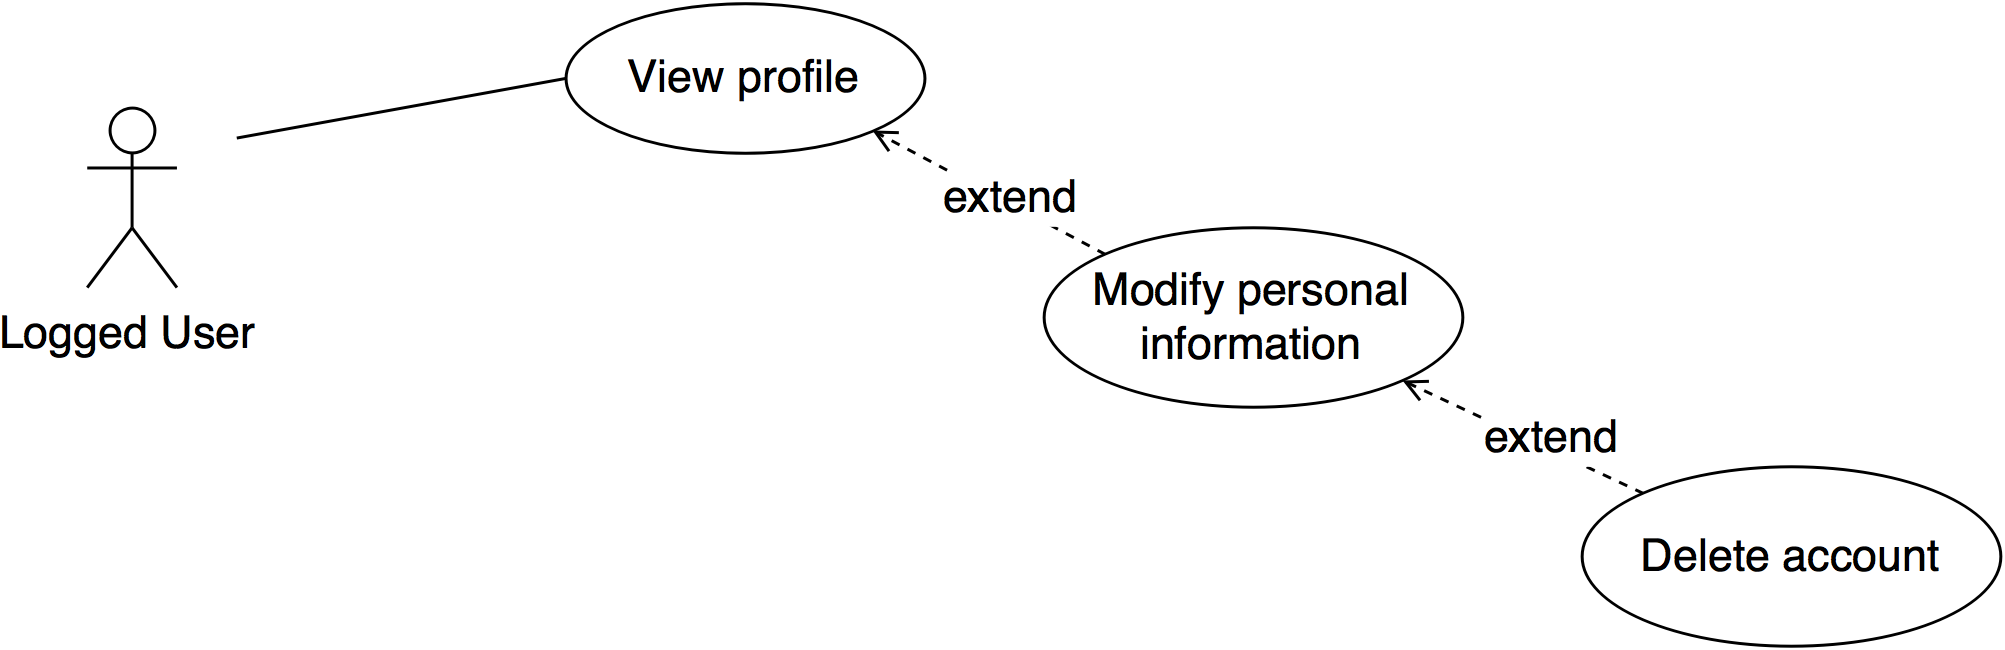
\includegraphics[width=\textwidth]{./specific_requirements/features/diagrams/man_profile_uc.png}
		\caption{Profile management use-case diagram}
		\label{man_profile_uc}
\end{center}
\end{figure}